
\section{Solutions for ``Permutations''}
\label{sec:AnswerKey:Permutations}
\noindent\textbf{\textit{ (Chapter \ref{Permutations})}}\bigskip


\noindent\textbf{Exercise \ref{exercise:Permutations:isos_tri_sym}:}
%Suppose that the two congruent sides of triangle $ABC$ are $\overline{AB}$ and $\overline{BC}$). Give the two symmetries, in tableau form.
\begin{multicols}{2}
\begin{itemize}
\item
$s = \begin{pmatrix}
A & B & C\\
C & B & A
\end{pmatrix}$

\item
$\var{id} = \begin{pmatrix}
A & B & C \\
A & B & C
\end{pmatrix}$
\end{itemize}
\end{multicols}

\noindent\textbf{Exercise \ref{exercise:Permutations:tri_sym}:}\\
%Suppose $T$ is used to represent any three-sided figure.  
%Which permutation(s) do(es) the set of symmetries of $T$ always contain?
$T = \{\var{id}\}$\\

\noindent\textbf{Exercise \ref{exercise:Permutations:S_4}:}
%Suppose $X = \{A, B, C, D\}$.
\begin{enumerate}[{a.}]
\item
%How many permutations are there on $X$?
Permutations = $4 \cdot 3 \cdot 2 \cdot 1 = 24$

\item
%List $S_X$.
	\begin{multicols}{3}
	\begin{itemize}
	\item
	$\begin{pmatrix}
	A & B & C & D\\
	A & B & C & D
	\end{pmatrix}$

	\item
	$\begin{pmatrix}
	A & B & C & D\\
	A & B & D & C
	\end{pmatrix}$
	
	\item
	$\begin{pmatrix}
	A & B & C & D\\
	A & C & B & D
	\end{pmatrix}$
	
	\item
	$\begin{pmatrix}
	A & B & C & D\\
	A & C & D & B
	\end{pmatrix}$
	
	\item
	$\begin{pmatrix}
	A & B & C & D\\
	A & D & B & C
	\end{pmatrix}$
	
	\item
	$\begin{pmatrix}
	A & B & C & D\\
	A & D & C & B
	\end{pmatrix}$
	
	\item
	$\begin{pmatrix}
	A & B & C & D\\
	B & A & C & D
	\end{pmatrix}$

	\item
	$\begin{pmatrix}
	A & B & C & D\\
	B & A & D & C
	\end{pmatrix}$
	
	\item
	$\begin{pmatrix}
	A & B & C & D\\
	B & C & A & D
	\end{pmatrix}$
	
	\item
	$\begin{pmatrix}
	A & B & C & D\\
	B & C & D & A
	\end{pmatrix}$
	
	\item
	$\begin{pmatrix}
	A & B & C & D\\
	B & D & A & C
	\end{pmatrix}$
	
	\item
	$\begin{pmatrix}
	A & B & C & D\\
	B & D & C & A
	\end{pmatrix}$
	
	\item
	$\begin{pmatrix}
	A & B & C & D\\
	C & A & B & D
	\end{pmatrix}$

	\item
	$\begin{pmatrix}
	A & B & C & D\\
	C & A & D & B
	\end{pmatrix}$
	
	\item
	$\begin{pmatrix}
	A & B & C & D\\
	C & B & A & D
	\end{pmatrix}$
	
	\item
	$\begin{pmatrix}
	A & B & C & D\\
	C & B & D & A
	\end{pmatrix}$
	
	\item
	$\begin{pmatrix}
	A & B & C & D\\
	C & D & A & B
	\end{pmatrix}$
	
	\item
	$\begin{pmatrix}
	A & B & C & D\\
	C & D & B & A
	\end{pmatrix}$
	
	\item
	$\begin{pmatrix}
	A & B & C & D\\
	D & A & B & C
	\end{pmatrix}$

	\item
	$\begin{pmatrix}
	A & B & C & D\\
	D & A & C & B
	\end{pmatrix}$
	
	\item
	$\begin{pmatrix}
	A & B & C & D\\
	D & B & A & C
	\end{pmatrix}$
	
	\item
	$\begin{pmatrix}
	A & B & C & D\\
	D & B & C & A
	\end{pmatrix}$
	
	\item
	$\begin{pmatrix}
	A & B & C & D\\
	D & C & A & B
	\end{pmatrix}$
	
	\item
	$\begin{pmatrix}
	A & B & C & D\\
	D & C & B & A
	\end{pmatrix}$
	\end{itemize}
	\end{multicols}
	
\item
%List the elements in $S_X$ that are not symmetries of the square.
	\begin{multicols}{3}
	\begin{itemize}
	\item
	$\begin{pmatrix}
	A & B & C & D\\
	A & B & D & C
	\end{pmatrix}$
	
	\item
	$\begin{pmatrix}
	A & B & C & D\\
	A & C & B & D
	\end{pmatrix}$
	
	\item
	$\begin{pmatrix}
	A & B & C & D\\
	A & C & D & B
	\end{pmatrix}$
	
	\item
	$\begin{pmatrix}
	A & B & C & D\\
	A & D & B & C
	\end{pmatrix}$
	
	\item
	$\begin{pmatrix}
	A & B & C & D\\	
	B & A & C & D
	\end{pmatrix}$
	
	\item
	$\begin{pmatrix}
	A & B & C & D\\
	B & C & A & D
	\end{pmatrix}$
	
	\item
	$\begin{pmatrix}
	A & B & C & D\\
	B & D & A & C
	\end{pmatrix}$
	
	\item
	$\begin{pmatrix}
	A & B & C & D\\
	B & D & C & A
	\end{pmatrix}$
	
	\item
	$\begin{pmatrix}
	A & B & C & D\\
	C & A & B & D
	\end{pmatrix}$
	
	\item
	$\begin{pmatrix}
	A & B & C & D\\
	C & A & D & B
	\end{pmatrix}$
	
	\item
	$\begin{pmatrix}
	A & B & C & D\\
	C & B & D & A
	\end{pmatrix}$
	
	\item
	$\begin{pmatrix}
	A & B & C & D\\
	C & D & B & A
	\end{pmatrix}$
	
	\item
	$\begin{pmatrix}
	A & B & C & D\\
	D & A & C & B
	\end{pmatrix}$
	
	\item
	$\begin{pmatrix}
	A & B & C & D\\
	D & B & A & C
	\end{pmatrix}$

	\item
	$\begin{pmatrix}
	A & B & C & D\\
	D & B & C & A
	\end{pmatrix}$
	
	\item
	$\begin{pmatrix}
	A & B & C & D\\
	D & C & A & B
	\end{pmatrix}$
	\end{itemize}
	\end{multicols}
	
\item
%What additional elements in $S_X$ are not symmetries of the rectangle?
	\begin{multicols}{3}
	\begin{itemize}
	\item
	$\begin{pmatrix}
	A & B & C & D\\
	A & D & C & B
	\end{pmatrix}$
	
	\item
	$\begin{pmatrix}
	A & B & C & D\\
	B & C & D & A
	\end{pmatrix}$
	
	\item
	$\begin{pmatrix}
	A & B & C & D\\
	C & B & A & D
	\end{pmatrix}$
	
	\item
	$\begin{pmatrix}
	A & B & C & D\\
	D & A & B & C
	\end{pmatrix}$
	\end{itemize}
	\end{multicols}
\end{enumerate}


\noindent\textbf{Exercise \ref{exercise:Permutations:7}:}
\begin{enumerate}[{a.}]
\item
%Write $\mu \compose \sigma$ in tableau form.
$\mu\circ\sigma=\begin{pmatrix}
A & B & C & D\\
D & C & B & A
\end{pmatrix}\circ\begin{pmatrix}
A & B & C & D\\
C & D & A & B
\end{pmatrix}=\begin{pmatrix}
A & B & C & D\\
B & A & D & C
\end{pmatrix}$

\item
%Write $\tau \compose \rho$ in tableau form.
$\tau\circ\rho=\begin{pmatrix}
1 & 2 & 3 & 4\\
4 & 3 & 2 & 1
\end{pmatrix}\circ\begin{pmatrix}
1 & 2 & 3 & 4\\
3 & 4 & 1 & 2
\end{pmatrix}=\begin{pmatrix}
1 & 2 & 3 & 4\\
2 & 1 & 4 & 3
\end{pmatrix}$

\item
%Is $ \mu \compose \sigma$ equivalent to $\tau \compose \rho$? \emph{Explain} your answer.
Yes, $\mu\circ\sigma$ is equivalent to $\tau\circ\rho$ because if we rename $A, B, C, D$ by $1, 2, 3, 4$, we will get the same result for both compositions.

\item
%Is $\sigma \compose \mu$ equivalent to $\rho \compose \tau$?  \emph{Explain} your answer.
Yes, you are just using substitution.
\end{enumerate}

\noindent\textbf{Exercise \ref{exercise:Permutations:isomorphic1}:} 
%Let $W =\{G, H \}$ and $Z = \{J, K \}$.
\begin{enumerate}[(a)]
\item
%Write the Cayley Tables for $S_W$ and $S_Z$. It would be helpful to write the entries of $S_W$ and $S_Z$ in tableau form. 
$|S_W| = 2$; $|S_Z| = 2$\\
	\begin{multicols}{2}
	\begin{itemize}
	\item
	$\sigma_1 = \begin{pmatrix}
	G & H\\
	G & H
	\end{pmatrix}$

	\item
	$\tau_1 = \begin{pmatrix}
	J & K\\
	J & K
	\end{pmatrix}$

	\item
	$\sigma_2 = \begin{pmatrix}
	G & H\\
	H & G
	\end{pmatrix}$

	\item
	$\tau_2 = \begin{pmatrix}
	J & K\\
	K & J
	\end{pmatrix}$\\	
	\end{itemize}
	\end{multicols}
	
	\begin{multicols}{2}
	\begin{tabular}{c| c c }
		o & $\sigma_1$ & $\sigma_2$\\
		\hline
		$\sigma_1$ & $\sigma_1$ & $\sigma_2$\\
		$\sigma_2$ & $\sigma_2$ & $\sigma_1$\\
	\end{tabular}

	\begin{tabular}{c| c c }
		o & $\tau_1$ & $\tau_2$ \\
		\hline
		$\tau_1$ & $\tau_1$ & $\tau_2$\\
		$\tau_2$ & $\tau_2$ & $\tau_1$\\
	\end{tabular}
	\end{multicols}
	
\item
%Give a bijection from $W$ to $Z$, and the corresponding bijection from $S_W$ to $S_Z$, that would show $S_W$ is isomorphic to $S_Z$. (Remember that a bijection can be thought of as  a ``relabeling'' of elements of $W$ as elements of $Z$.)
Bijection from $W\rightarrow Z$:
$f = \begin{pmatrix}
G & H\\
J & K
\end{pmatrix}$\\
\\
Bijection from $S_W \rightarrow S_Z = \begin{pmatrix}
\sigma_1 & \sigma_2\\
\tau_1 & \tau_2 
\end{pmatrix}$

\item
%*How many possible bijections from $W$ to $Z$ give rise to isomorphisms from  $S_W$ to  $S_Z$?
There are 2 possible bijections.
\end{enumerate}

\noindent\textbf{Exercise \ref{exercise:Permutations:11}:} %KW added d, a-c were UG
%Let $X =\{A, B, C\}$ and $Y = \{M, N, P\}$.
\begin{enumerate}[{a.}]
\item
%Write the Cayley Tables for $S_X$ and $S_Y$
$|S_X| = 6$; $|S_Y| = 6$\\
	\begin{multicols}{2}
	\begin{itemize}
	\item
	$\sigma_1 = \begin{pmatrix}
	A & B & C\\
	A & B & C
	\end{pmatrix}$

	\item
	$\tau_1 = \begin{pmatrix}
	M & N & P\\
	M & N & P
	\end{pmatrix}$

	\item
	$\sigma_2 = \begin{pmatrix}
	A & B & C\\
	B & C & A
	\end{pmatrix}$

	\item
	$\tau_2 = \begin{pmatrix}
	M & N & P\\
	N & P & M
	\end{pmatrix}$
	
	\item
	$\sigma_3 = \begin{pmatrix}
	A & B & C\\
	C & A & B
	\end{pmatrix}$

	\item
	$\tau_3 = \begin{pmatrix}
	M & N & P\\
	P & M & N
	\end{pmatrix}$\\

	\item
	$\sigma_4 = \begin{pmatrix}
	A & B & C\\
	A & C & B
	\end{pmatrix}$

	\item
	$\tau_4 = \begin{pmatrix}
	M & N & P\\
	M & P & N
	\end{pmatrix}$\\

	\item
	$\sigma_5 = \begin{pmatrix}
	A & B & C\\
	B & A & C
	\end{pmatrix}$

	\item
	$\tau_5 = \begin{pmatrix}
	M & N & P\\
	N & M & P
	\end{pmatrix}$\\

	\item
	$\sigma_6 = \begin{pmatrix}
	A & B & C\\
	C & B & A
	\end{pmatrix}$

	\item
	$\tau_6 = \begin{pmatrix}
	M & N & P\\
	P & N & M
	\end{pmatrix}$\\
	\end{itemize}
	\end{multicols}
	
	\begin{multicols}{2}
	\begin{tabular}{c| c c c c c c}
		o & $\sigma_1$ & $\sigma_2$ & $\sigma_3$ & $\sigma_4$ & $\sigma_5$ & $\sigma_6$\\
		\hline
		$\sigma_1$ & $\sigma_1$ & $\sigma_2$ & $\sigma_3$ & $\sigma_4$ & $\sigma_5$ & $\sigma_6$\\
		$\sigma_2$ & $\sigma_2$ & $\sigma_3$ & $\sigma_1$ & $\sigma_5$ & $\sigma_6$ & $\sigma_4$\\
		$\sigma_3$ & $\sigma_3$ & $\sigma_1$ & $\sigma_2$ & $\sigma_6$ & $\sigma_4$ & $\sigma_5$\\
		$\sigma_4$ & $\sigma_4$ & $\sigma_6$ & $\sigma_5$ & $\sigma_1$ & $\sigma_3$ & $\sigma_2$\\
		$\sigma_5$ & $\sigma_5$ & $\sigma_4$ & $\sigma_6$ & $\sigma_2$ & $\sigma_1$ & $\sigma_3$\\
		$\sigma_6$ & $\sigma_6$ & $\sigma_5$ & $\sigma_4$ & $\sigma_3$ & $\sigma_2$ & $\sigma_1$\\
	\end{tabular}

	\begin{tabular}{c| c c c c c c}
		o & $\tau_1$ & $\tau_2$ & $\tau_3$ & $\tau_4$ & $\tau_5$ & $\tau_6$\\
		\hline
		$\tau_1$ & $\tau_1$ & $\tau_2$ & $\tau_3$ & $\tau_4$ & $\tau_5$ & $\tau_6$\\
		$\tau_2$ & $\tau_2$ & $\tau_3$ & $\tau_1$ & $\tau_5$ & $\tau_6$ & $\tau_4$\\
		$\tau_3$ & $\tau_3$ & $\tau_1$ & $\tau_2$ & $\tau_6$ & $\tau_4$ & $\tau_5$\\
		$\tau_4$ & $\tau_4$ & $\tau_6$ & $\tau_5$ & $\tau_1$ & $\tau_3$ & $\tau_2$\\
		$\tau_5$ & $\tau_5$ & $\tau_4$ & $\tau_6$ & $\tau_2$ & $\tau_1$ & $\tau_3$\\
		$\tau_6$ & $\tau_6$ & $\tau_5$ & $\tau_4$ & $\tau_3$ & $\tau_2$ & $\tau_1$\\
	\end{tabular}
	\end{multicols}
	
\item
%Give a bijection from $X$ to $Y$, and the corresponding bijection from $S_X$ to $S_Y$, that would show $S_X$ is isomorphic to $S_Y$.
Bijection from $X\implies Y$:
$f = \begin{pmatrix}
A & B & C\\
M & N & P
\end{pmatrix}$\\
\\
Bijection from $S_X \implies S_Y = \begin{pmatrix}
\sigma_1 & \sigma_2 & \sigma_3 & \sigma_4 & \sigma_5 & \sigma_6\\
\tau_1 & \tau_2 & \tau_3 & \tau_4 & \tau_5 & \tau_6
\end{pmatrix}$

\item
%*How many possible bijections from $X$ to $Y$ produce isomorphisms from $S_X$ to $S_Y$?
There are 6 possible bijections.

\item
%*Now let $X =\{A, B, \ldots M\}$ and $Y = \{N, O, \ldots Z\}$. How many different bijections from $X$ to $Y$ produce isomorphisms from $S_X$ to $S_Y$?
There would be $13!=6,227,020,800$ bijections.
\end{enumerate}

\noindent\textbf{Exercise \ref{exercise:Permutations:permute_S5}:}
%Consider the subset $G$ of $S_5$ consisting of the identity
%permutation ${\var id}$ and the permutations 
%\begin{align*}
%\sigma
%& =
%\begin{pmatrix}
%1 & 2 & 3 & 4 & 5 \\
%1 & 2 & 3 & 5 & 4
%\end{pmatrix} \\
%\tau
%& =
%\begin{pmatrix}
%1 & 2 & 3 & 4 & 5 \\
%3 & 2 & 1 & 4 & 5
%\end{pmatrix} \\
%\mu
%& =
%\begin{pmatrix}
%1 & 2 & 3 & 4 & 5 \\
%3 & 2 & 1 & 5 & 4
%\end{pmatrix}.
%\end{align*}
\begin{enumerate}[{a.}]
\item
%Write the Cayley table for $G$ (Label your rows and columns as: ${\var id}, \sigma, \tau, \mu$).
\begin{tabular}{c| c c c c c c}
		o & $\var{id}$ & $\sigma$ & $\tau$ & $\mu$\\ \hline
		$\var{id}$ & $\var{id}$ & $\sigma$ & $\tau$ & $\mu$\\
		$\sigma$ & $\sigma$ & $\var{id}$ & $\mu$ & $\tau$\\
		$\tau$ & $\tau$ & $\mu$ & $\var{id}$ & $\sigma$\\
		$\mu$ & $\mu$ & $\tau$ & $\sigma$ & $\var{id}$\\
\end{tabular}

\item
%Use the Cayley table to explain whether $G$ is a subgroup of $S_5$ or not.  
%\medskip
%\emph{Remember: you don't need to show the associative property, since function composition is associative.}
Yes, $G$ is a subgroup of $S_5$, because $G$ is a group.  $G$ has an identity element, every element has an inverse, and $G$ is closed under $\circ$, so this proves $G$ is a group.
\end{enumerate}

\noindent\textbf{Exercise \ref{exercise:Permutations:permute_S4}:}
%Consider the subset $G$ of $S_4$ consisting of the identity
%permutation ${\var id}$ and the permutations 
%\begin{align*}
%\sigma
%& =
%\begin{pmatrix}
%1 & 2 & 3 & 4  \\
%2 & 3 & 1 & 4
%\end{pmatrix} \\
%\tau
%& =
%\begin{pmatrix}
%1 & 2 & 3 & 4  \\
%3 & 2 & 1 & 4 
%\end{pmatrix} \\
%\mu
%& =
%\begin{pmatrix}
%1 & 2 & 3 & 4  \\
%3 & 1 & 2 & 4 
%\end{pmatrix}.
%\end{align*}
\begin{enumerate}[{a.}]
\item
%Write the Cayley table for $G$ (Label your rows and columns as: ${\var id}, \sigma, \tau, \mu$).
\begin{tabular}{c| c c c c}
		o & $\var{id}$ & $\sigma$ & $\tau$ & $\mu$\\
		\hline
		$\var{id}$ & $\var{id}$ & $\sigma$ & $\tau$ & $\mu$\\
		$\sigma$ & $\sigma$ & $\mu$ & $\sigma\circ\tau$ & $\var{id}$\\
		$\tau$ & $\tau$ & $\tau\circ\sigma$ & $\var{id}$ & $\tau\circ\mu$\\
		$\mu$ & $\mu$ & $\var{id}$ & $\mu\circ\tau$ & $\sigma$\\
	\end{tabular}
	
\item
%Use the Cayley table to explain whether or not $G$ is a subgroup of $S_4$.
No, $G$ is not a subgroup of $S_4$, because $G$ is not closed under $\circ$, and therefore $G$ is not a group.
\end{enumerate}

\noindent\textbf{Exercise \ref{exercise:Permutations:equal_cycles2}:}\\
%Show that $(123456) = (345612)$ by drawing a figure similar to Figure~\ref{fig:cycle}  for each cycle.
\begin{multicols}{2}
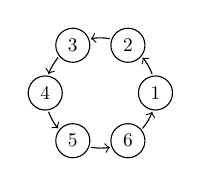
\begin{tikzpicture}[->,scale=.7]
   \node (1) at (0:1cm)  {$1$};
   \node (2) at (60:1cm) {$2$};
   \node (3) at (120:1cm) {$3$};
	\node (4) at (180:1cm)  {$4$};
   \node (5) at (240:1cm) {$5$};
   \node (6) at (300:1cm) {$6$};

   \draw (20:1cm)  arc (20:40:1cm);
   \draw (80:1cm) arc (80:100:1cm);
   \draw (140:1cm) arc (140:160:1cm);
   \draw (200:1cm)  arc (200:220:1cm);
   \draw (260:1cm) arc (260:280:1cm);
   \draw (320:1cm) arc (320:340:1cm);
\end{tikzpicture}

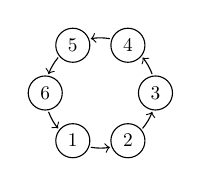
\begin{tikzpicture}[->,scale=.7]
   \node (1) at (0:1cm)  {$3$};
   \node (2) at (60:1cm) {$4$};
   \node (3) at (120:1cm) {$5$};
	\node (4) at (180:1cm)  {$6$};
   \node (5) at (240:1cm) {$1$};
   \node (6) at (300:1cm) {$2$};

   \draw (20:1cm)  arc (20:40:1cm);
   \draw (80:1cm) arc (80:100:1cm);
   \draw (140:1cm) arc (140:160:1cm);
   \draw (200:1cm)  arc (200:220:1cm);
   \draw (260:1cm) arc (260:280:1cm);
   \draw (320:1cm) arc (320:340:1cm);
\end{tikzpicture}
\end{multicols}

\noindent\textbf{Exercise \ref{exercise:Permutations:equal_cycles1}:}\\
%Show that $(123456)$  and $(234561)$ both have the same tableau (so they are in fact the same permutation).
\begin{multicols}{2}
$(123456) = \begin{pmatrix}
1 & 2 & 3 & 4 & 5 & 6\\
2 & 3 & 4 & 5 & 6 & 1
\end{pmatrix}$\\
\\
$(234561) = \begin{pmatrix}
1 & 2 & 3 & 4 & 5 & 6\\
2 & 3 & 4 & 5 & 6 & 1
\end{pmatrix}$\\
\end{multicols}

\noindent\textbf{Exercise \ref{exercise:Permutations:long_cycle_perm1}:}\\
%Write the following permutation of $S_6$ in cycle notation:  
%\[ \mu = \begin{pmatrix} 1 & 2 & 3 & 4 & 5 & 6 \\ 3 & 4 & 5 & 1 & 6 & 2 \end{pmatrix}. \]
$(135624)$\\
\\

\noindent\textbf{Exercise \ref{exercise:Permutations:long_cycle_perm2}:}
%Given the permutation $\mu = (152634)$ in $S_6$ :
\begin{enumerate}[(a)]
\item
%Write $\mu$ in tableau form.
$\mu = \begin{pmatrix}
1 & 2 & 3 & 4 & 5 & 6\\
5 & 6 & 4 & 1 & 2 & 3
\end{pmatrix}$

\item
%Write $\mu$ as a figure similar to Figure~\ref{fig:cycle}
$(152634)$\\
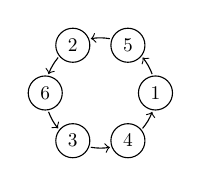
\begin{tikzpicture}[->,scale=.7]
   \node (1) at (0:1cm)  {$1$};
   \node (2) at (60:1cm) {$5$};
   \node (3) at (120:1cm) {$2$};
	\node (4) at (180:1cm)  {$6$};
   \node (5) at (240:1cm) {$3$};
   \node (6) at (300:1cm) {$4$};

   \draw (20:1cm)  arc (20:40:1cm);
   \draw (80:1cm) arc (80:100:1cm);
   \draw (140:1cm) arc (140:160:1cm);
   \draw (200:1cm)  arc (200:220:1cm);
   \draw (260:1cm) arc (260:280:1cm);
   \draw (320:1cm) arc (320:340:1cm);
\end{tikzpicture}
\end{enumerate}

\noindent\textbf{Exercise \ref{exercise:Permutations:long_cycle_perm3}:}
%Given the permutation in $S_6$ $\mu = (165432)$:
\begin{enumerate}[{a.}]
\item
%Write $\mu$ in tableau form.
$\mu = \begin{pmatrix}
1 & 2 & 3 & 4 & 5 & 6\\
6 & 1 & 2 & 3 & 4 & 5
\end{pmatrix}$

\item
%Write $\mu$ as a figure similar to Figure~\ref{fig:cycle}
$(165432)$\\
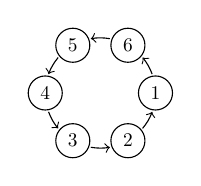
\begin{tikzpicture}[->,scale=.7]
   \node (1) at (0:1cm)  {$1$};
   \node (2) at (60:1cm) {$6$};
   \node (3) at (120:1cm) {$5$};
	\node (4) at (180:1cm)  {$4$};
   \node (5) at (240:1cm) {$3$};
   \node (6) at (300:1cm) {$2$};

   \draw (20:1cm)  arc (20:40:1cm);
   \draw (80:1cm) arc (80:100:1cm);
   \draw (140:1cm) arc (140:160:1cm);
   \draw (200:1cm)  arc (200:220:1cm);
   \draw (260:1cm) arc (260:280:1cm);
   \draw (320:1cm) arc (320:340:1cm);
\end{tikzpicture}

\item
%Compare your answer to (b) with Figure~\ref{fig:cycle} of $\rho = (123456)$.  Explain the difference between $\mu$ and $\rho$. 
$\rho$ expresses a reverse order of $\mu$
\end{enumerate}

\noindent\textbf{Exercise \ref{exercise:Permutations:short_cycle1}:}
%Write each of the following permutations in $S_7$ in tableau form.
\begin{multicols}{2}
\begin{enumerate}[{a.}]
\item
%$\omega = (243)$
$\omega = \begin{pmatrix}
1 & 2 & 3 & 4 & 5 & 6 & 7\\
1 & 4 & 2 & 3 & 5 & 6 & 7
\end{pmatrix}$

\item
%$\omega = (2365)$
$\omega = \begin{pmatrix}
1 & 2 & 3 & 4 & 5 & 6 & 7\\
1 & 3 & 6 & 4 & 2 & 5 & 7
\end{pmatrix}$

\item
%$\omega = (14257)$
$\omega = \begin{pmatrix}
1 & 2 & 3 & 4 & 5 & 6 & 7\\
4 & 5 & 3 & 2 & 7 & 6 & 1
\end{pmatrix}$
\end{enumerate}
\end{multicols}

\noindent\textbf{Exercise \ref{exercise:Permutations:short_cycle2}:}
%Draw a figure similar to Figure~\ref{fig:cycle} depicting each of the following permutations in $S_5$.
\begin{multicols}{3}
\begin{enumerate}[{a.}]
\item
%$\sigma = (25)$
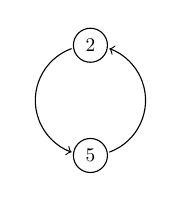
\begin{tikzpicture}[->,scale=.7]
   \node (1) at (90:1cm)  {$2$};
   \node (2) at (270:1cm) {$5$};
 
   \draw (-70:1cm)  arc (-70:70:1cm);
   \draw (110:1cm) arc (110:250:1cm);
\end{tikzpicture}

\item
%$\sigma = (135)$
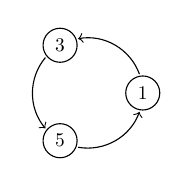
\begin{tikzpicture}[->,scale=.7]
   \node (1) at (0:1cm)  {$1$};
   \node (2) at (120:1cm) {$3$};
   \node (3) at (240:1cm) {$5$};
	
   \draw (20:1cm)  arc (20:100:1cm);
   \draw (140:1cm) arc (140:220:1cm);
   \draw (260:1cm) arc (260:340:1cm);
\end{tikzpicture}

\item
%$\sigma = (1342)$
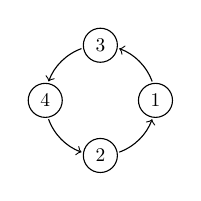
\begin{tikzpicture}[->,scale=.7]
   \node (1) at (0:1cm)  {$1$};
   \node (2) at (90:1cm) {$3$};
   \node (3) at (180:1cm) {$4$};
	\node (4) at (270:1cm)  {$2$};

   \draw (20:1cm)  arc (20:70:1cm);
   \draw (110:1cm) arc (110:160:1cm);
   \draw (200:1cm) arc (200:250:1cm);
   \draw (290:1cm)  arc (290:340:1cm);
  \end{tikzpicture}
\end{enumerate}
\end{multicols}

\noindent\textbf{Exercise \ref{exercise:Permutations:perm_not_comm}:}\\
%Using the same permutations $\sigma$ and $\tau$ as above:
$\sigma = (1532)$ and $\tau = (126)$
\begin{enumerate}[{a.}]
\item
%Write the product $\tau \sigma$ in cycle notation.
$\tau\sigma = (1536)$

\item
%By comparing your results for $\sigma \tau$ and $\tau \sigma$, fill in the blank in the following statement:  In general, permutations do not $\_\_\_\_\_\_\_\_\_\_\_\_$.
$\sigma\tau = (2653)$\\
commute
\end{enumerate}

\noindent\textbf{Exercise \ref{exercise:Permutations:cycle_comp_exer1}:}
%Given that $\delta = (135)$, $\sigma = (347)$, and $\rho = (567)$ are permutations in $S_7$, compute the following:
\begin{multicols}{2}
\begin{enumerate}[{a.}]
\item
$\delta \sigma = (135)(347) = (13475)$

\item
$\sigma \delta = (347)(135) = (14735)$

\item
$\delta \rho = (135)(567) = (13567)$

\item
$\rho \delta = (567)(135) = (13675)$

\item
%$\sigma \rho$

\item
$\rho \sigma = (567)(347) = (34567)$
\end{enumerate}
\end{multicols}

\noindent\textbf{Exercise \ref{exercise:Permutations:permute_disjoint}:}\\

\noindent\textbf{Exercise \ref{exercise:Permutations:tab_to_cycle}:} %KW added d
%Write the following permutations in cycle notation.
\begin{multicols}{2}
\begin{enumerate}[{a.}]
 
\item
%$ \rho =
%\begin{pmatrix}
%1 & 2 & 3 & 4 & 5 & 6  \\
%2 & 1 & 5 & 6 & 3 & 4 
%\end{pmatrix}$
$\rho = (12)(35)(46)$

\item
%$ \sigma =
%\begin{pmatrix}
%1 & 2 & 3 & 4 & 5 & 6\\
%2 & 5 & 6 & 4 & 1 & 3
%\end{pmatrix}$
$\sigma = (125)(36)$

\item
%$ \omega =
%\begin{pmatrix}
%1 & 2 & 3 & 4 & 5 & 6 \\
%4 & 5 & 1 & 6 & 2 & 3
%\end{pmatrix}$
$\omega = (1463)(25)$

\item
%$ \tau =
%\begin{pmatrix}
%1 & 2 & 3 & 4 & 5 & 6 \\
%5 & 3 & 4 & 1 & 2 & 6
%\end{pmatrix}
%$
$\tau = (15234)$
\end{enumerate}
\end{multicols}

\noindent\textbf{Exercise \ref{exercise:Permutations:cycle_to_tab}:} %KW added c
%Write each of the following permutations in $S_9$ in tableau form.
\begin{enumerate}[(a)]
\item
%$\mu = (259)(347)$.
$\mu = \begin{pmatrix}
1 & 2 & 3 & 4 & 5 & 6 & 7 & 8 & 9\\
1 & 5 & 4 & 7 & 9 & 6 & 3 & 8 & 2
\end{pmatrix}$

\item
%$\sigma = (25678)(14)(39)$.
$\sigma = \begin{pmatrix}
1 & 2 & 3 & 4 & 5 & 6 & 7 & 8 & 9\\
4 & 5 & 9 & 1 & 6 & 7 & 8 & 2 & 3
\end{pmatrix}$

\item
%$\tau = (286)(193)(457)$.
$\tau= \begin{pmatrix} 
1 & 2 & 3 & 4 & 5 & 6 & 7 & 8 & 9\\
9 & 8 & 1 & 5 & 7 & 2 & 4 & 6 & 3
\end{pmatrix}$

\item
%$\omega = (257)(18)$.
\end{enumerate}

\noindent\textbf{Exercise \ref{exercise:Permutations:D6_cycles}:}\\ %KW added
%Write the permutations of $D_6$ in cycle notation (recall that $D_6$ is the group of symmetries of a hexagon).
$(1), (135)(246), (14)(25)(36), (153)(264), (26)(35), (13)(46), \\(15(24), (12)(36)(45), (14)(23)(56), (16)(25)(34), (165432)$\\

\noindent\textbf{Exercise \ref{exercise:Permutations:D4_cycles}:}
%Write the symmetries of a square in cycle notation.
\begin{multicols}{3}
\begin{itemize}
\item
$\var{id}$

\item
$r_{90} = (1234)$

\item
$r_{180} = (13)(24)$

\item
$r_{270} = (1432)$

\item
$s_v = (14)(23)$

\item
$s_h = (12)(34)$

\item
$s_{45} = (13)$

\item
$s_{135} = (24)$
\end{itemize}
\end{multicols}

\noindent\textbf{Exercise \ref{exercise:Permutations:dis_cycles_comm}:}  %KW updated e
%In parts (a)--(d) below, write both permutations on the set $\{1,2,3,4,5,6\}$ in tableau form.
\begin{multicols}{2}
\begin{enumerate}[{a.}]
\item
%$(123)(45)$ and $(45)(123)$.
$(123)(45) = \begin{pmatrix}
1 & 2 & 3 & 4 & 5 & 6\\
2 & 3 & 1 & 5 & 4 & 6
\end{pmatrix}$

$(45)(123) = \begin{pmatrix}
1 & 2 & 3 & 4 & 5 & 6\\
2 & 3 & 1 & 5 & 4 & 6
\end{pmatrix}$

\item
%$(14)(263)$ and $(263)(14)$
$(14)(263) = \begin{pmatrix}
1 & 2 & 3 & 4 & 5 & 6\\
4 & 6 & 2 & 1 & 5 & 3
\end{pmatrix}$

$(263)(14) = \begin{pmatrix}
1 & 2 & 3 & 4 & 5 & 6\\
4 & 6 & 2 & 1 & 5 & 3
\end{pmatrix}$

\item
%$(1352)(46)$ and $(46)(1352)$
$(14)(263) = \begin{pmatrix}
1 & 2 & 3 & 4 & 5 & 6\\
3 & 1 & 5 & 6 & 2 & 4
\end{pmatrix}$

$(263)(14) = \begin{pmatrix}
1 & 2 & 3 & 4 & 5 & 6\\
3 & 1 & 5 & 6 & 2 & 4
\end{pmatrix}$

\item
%$(135)(246)$ and $(246)(135)$

\item
%From your results in (a)-(d), what do you conjecture about the product of disjoint cycles?
The product of two disjoint cycles is commutative. Given two disjoint cycles $\tau$ and $\rho, \tau\rho = \rho\tau$.
\end{enumerate}
\end{multicols}

\noindent\textbf{Exercise \ref{exercise:Permutations:disjoint_commutative}:}
%Fill in the blanks  to complete the proof:
%
%Recall that permutations are defined as bijections on a set $X$. In order to show that the two permutations 
%$\sigma \tau$ and $\tau \sigma$ are equal, it's enough to show that they are the same function. In other words, we just need to show that 
\begin{multicols}{5}
\begin{enumerate}
\item
%$\sigma \tau (x)$ =$\underline{ ~<1>~}$ for all $x \in X$.
$\tau\sigma(x)$

\item
%
%We'll define $A = \{a_1, a_2, \ldots, a_j\}$ and $B = \{b_1, b_2, \ldots, b_k\}$. By hypothesis $A$ and $B$ are disjoint, so $A \underline{ ~<2>~} 
$\cap$

\item
%B = \underline{ ~<3>~}$. 
$\emptyset$

\item
%Given an arbitrary $x \in X$, there are three possibilities: (i) $x \in A$ and $x \notin B$; (ii) $x \in \underline{ ~<4>~}$ 
$B$

\skipitems{1}

\item
%and $x \notin \underline{ ~<6>~}$; 
$A$

\item
%(iii) $x \notin \underline{ ~<7>~}$ 
$A$

\item
%and $x \notin \underline{ ~<8>~}$. 
$B$

\item
%
%\begin{enumerate}[(i)]
%\item
%In this case, since $x \notin B$ it follows that $\tau(x) = x$. We then have $\sigma \tau (x) = \sigma(\tau(x)) = \sigma(x)$. Furthermore, since $x \in A$ it follows that $\sigma(x) \in A$, so $\sigma(x) \notin B$. We then have $\tau \sigma (x) = \tau(\sigma(x)) = \sigma(x)$. It follows that $\sigma \tau (x) = \tau \sigma (x)$.
%\item
%In this case, since $x \notin \underline{ ~<9>~}$
$A$

\item
%it follows that $\underline{ ~<10>~}(x) = x$.
$\sigma$

\item
% We then have $\tau \sigma (x) = \underline{ ~<11>~} = 
$\tau(\sigma(x))$

\item
%\underline{ ~<12>~}(x)$. 
$\tau(x)$

\item
%Furthermore, since $x \in \underline{ ~<13>~}$ 
$B$

\item
%it follows that $\underline{ ~<14>~}(x) 
$\tau$

\item
%\in \underline{ ~<15>~}$, 
$B$

\item
%so $\underline{ ~<16>~}(x) 
$\tau(x)$

\item
%\notin \underline{ ~<17>~}$.
$A$

\item
% We then have $\sigma \tau (x) = \underline{ ~<18>~} = 
$\sigma(\tau(x))$

\item
%\underline{ ~<19>~}(x)$. 
$\tau$

\item
%It follows that $\sigma \tau (x) = \tau \sigma (x)$.
%\item
%In this case, since $x \notin A$ it follows that $\underline{ ~<20>~}(x) =
$\sigma$

\item
% x$. Similarly since $x \notin \underline{ ~<21>~}$ 
$B$

\item
%it follows that $\underline{ ~<22>~}(x) = 
$\tau$

\item
%x$.We then have $\tau \sigma (x) = \underline{ ~<23>~}$ 
$x$

\item
%and $\sigma \tau (x) = \underline{ ~<24>~}$. 
$x$

\item
%It follows that $\sigma \tau (x) = \tau \sigma (x)$.
%\end{enumerate}
%
%\noindent
%In all three cases we have $\sigma \tau (x)$ = $\underline{ ~<25>~}$,
$\tau\sigma(x)$
% so therefore $\sigma \tau = \tau \sigma$.
\end{enumerate}
\end{multicols}

\noindent\textbf{Exercise \ref{exercise:Permutations:disjoint_commute_tableau}:}\\

\noindent\textbf{Exercise \ref{exercise:Permutations:disjoint_commute_cycle}:}\\

\noindent\textbf{Exercise \ref{exercise:Permutations:cycle_comp_5}:}
%Given the following permutations in $S_8$, 
%
%\[  \sigma = (1257)(34) , \tau = (265)(137), \text { and } \rho = (135)(246)(78) \]
%
%\noindent
%find the products:
\begin{enumerate}[{a.}]
\item
$\sigma\tau = [(1257)(34)][(265)(137)] = (143)(267)$

\item
$\tau \sigma = [(265)(137)][(1257)(34)] = (165)(347)$

\item
$\tau \rho = [(265)(137)][(135)(246)(78)] = (178)(2453)$

\item
$\sigma \rho = (1257)(34)(135)(246)(78) = (14652378)$
\end{enumerate}

\noindent\textbf{Exercise \ref{exercise:Permutations:cycle_comp_2}:} %KW added d
%Compute each of the following. Note that e.g. $(123)^2$ means the same as $(123)(123)$.
\begin{enumerate}[{a.}]
\item
$(1345)(234) = (135)(24)$

\item
$(12)(1253) = (253)$

\item

\item
$(1423)(34)(56)(132) = (124)(56)$

\item
$(1254)(13)(25)^2 = (13254)$ 

\item
$(1254)^2(123)(45) = (14)(235)$ 
\end{enumerate}

\noindent\textbf{Exercise \ref{exercise:Permutations:uniqueness_proof}:}\\

\noindent\textbf{Exercise \ref{exercise:Permutations:cycle_types}:} %KW added c
%Following Example~\ref{example:Permutations:S5_cycle_types}, list  all possible cycle structures of permutations in the following:
\begin{enumerate}[{a.}]
\item
%$S_6$
Types of permutations in $S_6$ are:
	\begin{itemize}
	\item
	The identity - no cycles
	
	\item
	Single cycles of lengths - 6, 5, 4, 3, and 2.
	
	\item
	4 sets of two disjoint cycles of lengths - 2 and 4; 2 and 3; 2 and 2; 3 and 3.
	
	\item
	1 set of three disjoint cycles of lengths - 2 and 2 and 2.
	\end{itemize}
	
\item
%$S_7$
Type of permutations in $S_7$ are:
	\begin{itemize}
	\item
	The identity - no cycle.
	
	\item
	Single cycles of lengths - 7, 6, 5, 4, 3, and 2.
	
	\item
	6 sets of two disjoint cycles of lengths - 2 and 5; 2 and 4; 2 and 3; 2 and 2; 3 and 4; 3 and 3.
	
	\item
	2 sets of three disjoint cycles of lengths - 2 and 2 and 2; 2 and 2 and 3.
	\end{itemize}

\item
%$S_8$
Type of permutations in $S_8$ are:
	\begin{itemize}
	\item
	The identity - no cycle.
	
	\item
	Single cycles of lengths - 8, 7, 6, 5, 4, 3, and 2.
	
	\item
	two disjoint cycles of lengths - 2 and 6; 2 and 5; 2 and 4; 2 and 3; 2 and 2; 3 and 5; 3 and 4; 3 and 3; 4 and 4.
	
	\item
	three disjoint cycles of lengths - 2, 2, and 4; 2, 2, and 3; 2, 2 and 2; 2, 3, and 3.
	
	\item
	four disjoint cycles of lengths - 2, 2, 2, and 2.
	\end{itemize}
\end{enumerate}

\noindent\textbf{Exercise \ref{exercise:Permutations:4th_power}:}
%Compute each of the following.
\begin{multicols}{3}
\begin{enumerate}[(a)]
\item
%$(1 2 6 4)^3$
$(1 2 6 4)^3 = (1462)$

\item
%$(1 2 6 4)^4$
$(1 2 6 4)^4 = \var{id}$

\item
%$(1 2 6 4)^5$
$(1 2 6 4)^5 = (1 2 6 4)$
\end{enumerate}
\end{multicols}

\noindent\textbf{Exercise \ref{exercise:Permutations:6th_power}:}
%Compute each of the following:
\begin{enumerate}[{a.}]
\begin{multicols}{2}
\item
$(125843)^2 = (154)(283)$

\item
$(125843)^3 = (18)(24)(35)$

\item
$(125843)^4 = (145)(238)$

\item
$(125843)^5 = (134852)$

\item
$(125843)^6 = \var{id}$

\item
$(125843)^7 = (125843)$
\end{multicols}
\end{enumerate}

\noindent\textbf{Exercise \ref{exercise:Permutations:power of n-cycle1}:} %KW updated
%Let $X = \{1,2,\ldots,10\}$, let $A = \{2,5,7,8\}$, and let $\sigma \in S_X$ be the cycle  $\sigma = ( 2 5 7 8 )$.
\begin{enumerate}[{a.}]
\item
%What is $\sigma(2)$? What is $\sigma^2(2)$? What is $\sigma^3(2)$? What is $\sigma^4(2)$ What is $\sigma^{3,482,991}(2)?$  
	\begin{itemize}
	\item
	$\sigma(2) = 5$
	
	\item
	$\sigma^2(2) = 7$
	
	\item
	$\sigma^3(2) = 8$
	
	\item
	$\sigma^4(2) = 2$
	
	\item
	$\sigma^{3,482,991}(2) = \sigma^{\bmod{(3,4)}}(2) = 8$
	\end{itemize}
	
\item
%What is $\sigma(5)$? What is $\sigma^2(5)$? What is $\sigma^3(5)$? What is $\sigma^4(5)$ What is $\sigma^{3,482,991}(5)?$  
	\begin{itemize}
	\item
	$\sigma(5) = 7$
	
	\item
	$\sigma^2(5) = 8$
	
	\item
	$\sigma^3(5) = 2$
	
	\item
	$\sigma^4(5) = 5$
	
	\item
	$\sigma^{3482991}(5) = \sigma^{\bmod{(3,4)}}(5) = 2$
	\end{itemize}
	
\item
%Fill in the blank: If $x \in A$ then $\sigma^k(x) = \sigma^{\bmod(k,\underline{~~})}$.
$\sigma^{\mod(k,4)}$

\item
%What is $\sigma(1)$? What is $\sigma(3)$? 
	\begin{itemize}
	\item
	$\sigma(1) = 1$
	
	\item
	$\sigma(3) = 3$
	\end{itemize}
	
\item
%What general statement can you make about $\sigma^k(x)$ for $x \in X \backslash A$?
$\sigma^k(x) = x$ for $x\in X\setminus A$

\item 
%** Let $K = \{k: \sigma^k(x) = x ~~\forall x \in X\}$. Is $2 \in K$?   Is $3 \in K$? Is $4 \in K$? Given any positive integer $k$, what's a simple way of telling whether or not $k \in K$?
Given any positive integer $k$, we can tell that $k \in K$, if $\mod(k,4) = 0$\\
$\therefore\ 2\not\in K, 3\not\in K, 4\in K$
\end{enumerate}

\noindent\textbf{Exercise \ref{exercise:Permutations:length_equals_order}:}
% Prove part (A) by filling in the blanks.
%
%\noindent
\begin{multicols}{3}
\begin{enumerate}
\item
%Let $\sigma \in S_X$ be an arbitrary cycle of length $k$.  Then $\sigma$ can be written as $ (a_1 \, a_2 \, \ldots \, a_k)$, for some set of elements $a_1, a_2, \ldots a_k$ in $X$.  In order to show that $\sigma^k = {\var id} $, it is sufficient to show that 
%$\sigma^k(x) = \underline{~<1>~}  \forall x \in X$. 
%Let $A$ be the set  $\{a_1, a_2, \ldots a_k\}$.  Now for any $x \in X$, there are two possibilities:  
%\begin{enumerate}[(i)]
%\item
%$x \in  X \backslash A$;
%\item
%$x \in A$. 
%\end{enumerate}
$x$

%\noindent
%We'll deal with these two cases separately (as we did  in Exercise~\ref{exercise:Permutations:power of n-cycle1}).
%
%\begin{enumerate}[(i)]
\item
%In this case, $\sigma(x) = \underline{~<2>~} $  
$x$

\item
%It follows that $\sigma^2(x) = \sigma( \sigma(x)) = \sigma( \underline{~<3>~}) 
$x$

\item
%= \underline{~<4>~}$. 
$x$

\item
%We can use the same argument to show that $\sigma^3(x) = \underline{~<5>~}$, 
$x$

\item
%and that $\sigma^k(x) = \underline{~<6>~}$ 
$x$

\item
%for any natural number $\underline{~<7>~}$.
$k$

\item
%In this case, then $x = a_j$ for some integer $j, 1 \le j \le \underline{~<8>~}$.  
$k$

\item
%It follows from the definition of cycle that $\sigma(x) = \sigma(a_j) = a_{\bmod(j+1,k)}$. Furthermore, $\sigma^2(x) = \sigma(a_{\bmod(j+1,k)}) = \underline{~<9>~}$. 
$a_{\bmod{(j+2,k)}}$

\item
%Similarly it follows that $\sigma^{k}(x) = a_{\bmod(j+ \underline{~<10>~},k)} 
$k$

\item
%= a_{\underline{~<11>~}} = x$.
$j$

\item
%\end{enumerate}
%
%\noindent
%Cases (i) and (ii) establish that  $\forall x \in X, \underline{~<12>~} 
$\sigma^k(x)$

\item
%= x$.  It follows that $\sigma^k = \underline{~<13>~}$.
$\var{id}$
\end{enumerate}
\end{multicols}

\noindent\textbf{Exercise \ref{exercise:Permutations:length_equals_order2}:}
% In this exercise we use the same notation as part (A), that is: $\sigma \in S_X$ has length $k$ and is represented as: $\sigma = (a_1 \, a_2 \, \ldots \, a_k)$. 
\begin{enumerate}[{a.}]
\item
%What is $\sigma(a_1)$? What is $\sigma^2(a_1)$? What is $\sigma^3(a_1)$? What is $\sigma^{k-1}(a_1)$?
	\begin{multicols}{3}
	\begin{itemize}
	\item
	$\sigma(a_1) = a_2$
	
	\item
	$\sigma^2(a_1) = a_3$
	
	\item
	$\sigma^3(a_1) = a_4$
	
	\item
	$\sigma^{k-1}(a_1) = a_k$
	\end{itemize}
	\end{multicols}
	
\item
%Conclude from part (a) that  $\sigma^j \neq {\var id} $ for $j = 1,2,3, \ldots, k-1.$
Proof by contradiction:
\\
Suppose $\sigma^j = \var{id}$ for $j < k$. Then $\sigma^{j(a_1)} = a_1$ by definition of $\var{id}$. But in part (a) we showed that $\sigma^{j(a_1)} \neq a_1$.  It follows that $\sigma^j \neq \var{id}$ for $j < k$. 
\end{enumerate}

\noindent\textbf{Exercise \ref{exercise:Permutations:cycle_order_1}:} %KW updated d
%Compute the following:
\begin{enumerate}[{a.}]
\item
$(1264)^{11} = [(1264)^4]^2(1264)^3 = \var{id}(1264)^3 = (1462)$

\item
$(125843)^{53} = (125843)^{mod(53,6)} = (125843)^5 = (134852)$

\item
$(352)(136)(1254)^{102} = (352)(136)(1254)^{mod(102,4)} = (12436)$

\item
$(348)(456)^5(1325)^{10} = (348)(456)^2(1325)^2 = (12)(38)(465)$
\end{enumerate}

\noindent\textbf{Exercise \ref{exercise:Permutations:64}:}
%Fill in the blanks with the appropriate variables in the following proof of the proposition.
%\hyperref[sec:Permutations:Hints]{(*Hint*)}
%\medskip
%
%\noindent
\begin{multicols}{5}
\begin{enumerate}
\item
%{\bf Proof:} For any integer $\ell$ we may write $\ell = ak + b$, where $b \in \mathbb{Z}_{\underline{~<1>~}} $. It follows that
$k$

\item
%\[ \tau^{\ell} = \tau^{<\underline{2}> \cdot k + 
$a$

\item
%<\underline{3}>} = 
$b$

\item
%(\tau^{<\underline{4}> \cdot k})
$a$

\item
%\tau^{<\underline{5}>} 
$b$

\item
%=   (\tau^k)^{<\underline{6}>}
$a$

\item
%\tau^{<\underline{7}>} 
$b$

\item
%= ({\var id})^{<\underline{8}>}
$a$

\item
%\tau^{<\underline{9}>} 
$b$

\item
%= \tau^{<\underline{10}>} . \]
$b$

\item
%Therefore $\tau^{\ell} = {\var id}$ if and only if $\tau^{<\underline{11}>} = {\var id}$. 
$b$

\item
%However, we know that $\underline{~<12>~} < k$, 
$b$

\item
%and we also know that $\underline{~<13>~}$ 
$k$

\item
%is the smallest positive integer such that  $\tau^{<\underline{14}>} 
$k$

\item
%= {\var id}$. Hence it must be the case that $b \equiv \underline{~<15>~} \bmod{k}$, 
$0$

\item
%which is the same thing as saying that  $\ell \equiv \underline{~<16>~}
$0$

\item
% \bmod{\underline{~<17>~}}$.
$k$
\end{enumerate}
\end{multicols}

\noindent\textbf{Exercise \ref{exercise:Permutations:disjoint_cube}:}
\begin{enumerate}[{a.}]
\item
%Let $\sigma = (237)$ and $\tau = (458)$. By following the format of Example~\ref{example:Permutations:disjoint_squared}, show that $(\sigma \tau)^3 = {\var id} $ (write out each step, and cite the property used).
\begin{align*}
(\sigma\tau)^3 &= [(237)(458)][(237)(458)][(237)(458)] &\text{(substitution)}
\\
&= (237)[(458)(237)][(458)(237)](458) &\text{(associative)}
\\
&= (237)[(237)(458)][(237)(458)](458) &\text{(commutative)}
\\
&= [(237)(237)][(458)(237)][(458)(458)] &\text{(associative)}
\\
&= [(237)(237)][(237)(458)][(458)(458)] &\text{(commutative)}
\\
&= [(237)(237)(237)][(458)(458)(458)] &\text{(associative)}
\\
&= (\var{id})(\var{id}) &\text{(3-cycles have order of 3, def. of\ } \var{id})
\\
&= \var{id} &\text{(def. of\ } \var{id})
\end{align*}

\item
%** If $\sigma$ and $\tau$ are disjoint cycles with $|\sigma| = |\tau| = k$, what may you conclude about $| \sigma \tau |$? (You don't need to give a proof).
If $|\sigma| = |\tau| = k$, then we can conclude that $|\sigma\tau| = k$.
\end{enumerate}

\noindent\textbf{Exercise \ref{exercise:Permutations:k_power_disjoint_cycles}:}
\begin{enumerate}[{a.}]
\item
%Let $\sigma$ and $\tau$ be \emph{any} disjoint cycles. By following the format of Example~\ref{example:Permutations:disjoint_squared}, show that $(\sigma \tau)^2 = \sigma^2 \tau^2$ (write out each step, and cite the property used).
\begin{align*}
(\sigma\tau)^2 &= (\sigma\tau)(\sigma\tau) &\text{(substitution)}
\\
&= \sigma(\tau\sigma)\tau &\text{(associative)}
\\
&= \sigma(\sigma\tau)\tau &\text{(commutative)}
\\
& =(\sigma\sigma)(\tau\tau) &\text{(associative)}
\\
& =\sigma^2\tau^2 &\text{(composition)}
\end{align*}

\item
%If $\sigma$ and $\tau$ are disjoint cycles and $k$ is a natural number, what may you conclude about $(\sigma \tau)^k$ in terms of powers of $\sigma$ and $\tau$? (You don't need to give a proof).
If $\sigma$ and $\tau$ are disjoint cycles and $k \in {\mathbb N}$, then $(\sigma\tau)^k = \sigma^k\tau^k$.
\end{enumerate}

\noindent\textbf{Exercise \ref{exercise:Permutations:disjoint_order_1}:}
%Suppose then $\tau = (1 2 3)( 4 5)$. Compute each of the following
\begin{enumerate}[{a.}]
\item 
$\tau^2 = (123)^2(45)^2 = (123)^2 = (132)$

\item 
$\tau^3 = (123)^3(45)^3 = (45)$

\item 
$\tau^4 = (123)^4(45)^4 = (123)$

\item 
$\tau^5 = (123)^5(45)^5 = (123)^2(45) = (132)(45)$

\item 
$\tau^6 =  (123)^6(45)^6 = \var{id}$

\item
$\tau^7 =  (123)^7(45)^7 = (123)(45)$
\end{enumerate}

\noindent\textbf{Exercise \ref{exercise:Permutations:Sn_orders}:} %KW updated
%What are all the possible orders for the permutations in each of the following sets (look back at your work for Exercise~\ref{exercise:Permutations:cycle_types}).
\begin{enumerate}[{a.}]
\item
%$S_6$
	\begin{multicols}{2}
	\begin{itemize}
	\item
	Length of single cycles - 2, 3, 4, 5, 6
	
	\item
	$\mbox{lcm}(2, 2) = 2$
	
	\item
	$\mbox{lcm}(2, 3) = 6$
	
	\item
	$\mbox{lcm}(2, 4) = 4$
	
	\item
	$\mbox{lcm}(3, 3) = 3$
	
	\item
	$\mbox{lcm}(2, 2, 2) = 2$
	\end{itemize}
	\end{multicols}
Possible orders of $S_6$ are: 2, 3, 4, 5, 6.
	
\item
%$S_7$
	\begin{multicols}{2}
	\begin{itemize}
	\item
	Length of single cycles - 2, 3, 4, 5, 6, 7
	
	\item
	$\mbox{lcm}(2, 2) = 2$
	
	\item
	$\mbox{lcm}(2, 3) = 6$
	
	\item
	$\mbox{lcm}(2, 4) = 4$
	
	\item
	$\mbox{lcm}(2, 5) = 10$
	
	\item
	$\mbox{lcm}(3, 3) = 3$
	
	\item
	$\mbox{lcm}(3, 4) = 12$
	
	\item
	$\mbox{lcm}(2, 2, 2) = 2$
	
	\item
	$\mbox{lcm}(2, 2, 3) = 6$
	\end{itemize}
	\end{multicols}
Possible orders of $S_7$ are: 2, 3, 4, 5, 6, 7, 10, 12.

\item
%$S_8$
\begin{multicols}{2}
	\begin{itemize}
	\item
	Length of single cycles - 2, 3, 4, 5, 6, 7, 8
	
	\item
	$\mbox{lcm}(2, 2) = 2$
	
	\item
	$\mbox{lcm}(2, 3) = 6$
	
	\item
	$\mbox{lcm}(2, 4) = 4$
	
	\item
	$\mbox{lcm}(2, 5) = 10$
	
	\item
	$\mbox{lcm}(2, 6) = 6$
	
	\item
	$\mbox{lcm}(3, 3) = 3$
	
	\item
	$\mbox{lcm}(3, 4) = 12$
	
	\item
	$\mbox{lcm}(3, 5) = 15$
	
	\item
	$\mbox{lcm}(4, 4) = 4$
	
	\item
	$\mbox{lcm}(2, 2, 2) = 2$
	
	\item
	$\mbox{lcm}(2, 2, 3) = 6$
	
	\item
	$\mbox{lcm}(2, 2, 4) = 4$
	
	\item
	$\mbox{lcm}(2, 3, 3) = 6$
	
	\item
	$\mbox{lcm}(2, 2, 2, 2) = 2$
	\end{itemize}
	\end{multicols}
Possible orders of $S_8$ are: 2, 3, 4, 6, 7, 8, 10, 12, 15.
\end{enumerate}

\noindent\textbf{Exercise \ref{exercise:Permutations:disjoint_order_2}:}
%Compute the following:
\begin{enumerate}[{a.}]
\item
$|(1254)^2| = |(15)(24)| \implies \mbox{lcm}(2, 2) = 2$ 

\item
$|(13658)^2(473)^2(125) = |(12)(374568)| \implies \mbox{lcm}(2, 6) = 6$

\item
$|(13658)^{13}(1254)^{11}(473)| = |(14786)(25)| \implies \mbox{lcm}(2, 5) = 10$

\item
$|(123456789)^{300}| = |(123456789)^3| = |(147)(258)(369)| \implies \mbox{lcm}(3, 3, 3) = 3$
\end{enumerate}

\noindent\textbf{Exercise \ref{exercise:Permutations:example_transpositions}:}
%Compute the following products:
\begin{enumerate}[{a.}]
\item
$(14)(13)(12) = (1234)$

\item
$(14)(18)(19) = (1984)$

\item
$(16)(15)(14)(13)(12) = (123456)$

\item
$(49)(48)(47)(46)(45) = (456789)$

\item

\end{enumerate}

\noindent\textbf{Exercise \ref{exercise:Permutations:example_transpositions2}:} %KW added f
%In light of what you discovered in the previous exercise, write each cycle as a product of transpositions:
\begin{enumerate}[{a.}]
\item
$(1492) = (12)(19)(14)$

\item
$(12345) = (15)(14)(13)(12)$

\item
$(472563) = (43)(46)(45)(42)(47)$

\item

\item
$(a_1a_2a_3a_5a_6) = (a_1a_6)(a_1a_5)(a_1a_3)(a_1a_2)$

\item
$(a_1 a_2 a_3 a_5 a_6 a_7 a_8) =  (a_1a_8)(a_1a_7)(a_1a_6)(a_1a_5)(a_1a_3)(a_1a_2)$
\end{enumerate}

\noindent\textbf{Exercise \ref{exercise:Permutations:prod_of_trans_1}:} %KW added f
%Express the following permutations as products of transpositions. 
\begin{enumerate}[{a.}]
\item
$(14356) = (16)(15)(13)(14)$

\item
$(156)(234) = (16)(15)(24)(23)$

\item

\item
$(17254)(1423)(154632) = (14672) = (12)(17)(16)(14)$

\item

\item
$( 1 3 5 7 9 )(2 4 6 8 ) (1 9 7 5 3) (2 8 6 4) = \var{id}$
\end{enumerate}

\noindent\textbf{Exercise \ref{exercise:Permutations:prod_of_trans_2}:}
%Compute the following products:
\begin{multicols}{2}
\begin{enumerate}[{a.}]
\item
$(12)(12) = \var{id}$

\item

\item
$(a_1 a_2)(a_1 a_2) = \var{id}$

\item
\end{enumerate}
\end{multicols}

\noindent\textbf{Exercise \ref{exercise:Permutations:inv_comps}:} %KW added f
%Calculate each of the following.
\begin{enumerate}[{a.}]    
\item
$(12537)^{-1} = (17352)$

\item
$[(12)(34)(12)(47)]^{-1} = (47)(12)(34)(12) = (374)$

\item
$[(1235)(467)]^{-2} = [(467)^{-1}(1235)^{-1}]^2 = [(476)(1532)]^2 = (467)(13)(25)$

\item
$(1254)^{-1}(123)(45)(1254) = (1452)(123)(45)(1254) = (134)(25)$

\item
$(123)(45)(1254)^{-2} = (123)(45)[(1254)^{-1}]^{2} = (123)(45)(1452)^{2} =  (143)(25)$

\item
$(742)^{-7}(286)^{-13} = [(742)^{-1}]^{7}[(286)^{-1}]^{13} = (724)^{7}(268)^{13} = (724)^{1}(268)^{1} = (724)(268) = (26847)$
\end{enumerate}

\noindent\textbf{Exercise \ref{exercise:Permutations:switchyard1}:} %KW added
%First we'll look at a switchyard with 4 positions.  As above, $r$ = counterclockwise rotation by 1 position = $(1 \, 2 \, 3 \, 4)$; while $t$  exchanges two cars: $t = (1 \, 2)$. 
\begin{enumerate}[(a)]
\item
%Write $(2 \, 3)$, $(3 \, 4)$, and $(4 \, 1)$ as products of powers of $r$ and $t$. (Together with $(1 \, 2)$, these are all the  consecutive 2-cycles.)
$(23)=r^{1}\circ t\circ r^{-1}$ \\
$(34)=r^{2}\circ t\circ r^{-2}$ \\
$(41)=r^{-1}\circ t\circ r^{1}$ 

\item
%Write $(1 \, 2 \, 3)$, $(2 \, 3 \, 4)$, $(3 \, 4 \, 1)$, $(4 \, 1 \, 2)$ as products of powers of $r$ and $t$. (These are all the counterclockwise consecutive  3-cycles.)
$(123)=(12)(23)=t\circ r\circ t\circ r^{-1}$ \\
$(234)=(23)(34)=r\circ t\circ r\circ t\circ r^{-2}$ \\
$(341)=(34)(41)=r^{2}\circ t\circ r\circ t\circ r$ 

\item
%Write $(1 \, 3 \, 2)$, $(2 \, 4 \, 3)$, $(3 \, 1 \, 4)$, $(4 \, 2 \, 1)$ as products of powers of $r$ and $t$. (These are all the clockwise consecutive 3-cycles.)
%\hyperref[sec:Permutations:Hints]{(*Hint*)}
$(132)=(23)(12)=r\circ t\circ r^{-1}\circ t$ \\
$(243)=(34)(23)=r^{2}\circ t\circ r^{-1}\circ t\circ r^{-1}$ \\
$(314)=(41)(34)=r^{-1}\circ t\circ r^{-1}\circ t\circ r^{-2}$ \\
$(421)=(12)(41)=t\circ r^{-1}\circ t\circ r$ 

\item
%Write $(1 \, 3)$ as products of powers of $r$ and $t$.
$(13)=t\circ r^{1}\circ t\circ r^{-1}\circ t$

\item
%Show that any transposition can be written as products of powers of $r$ and $t$.
Given $(12)=t$\\
from part $(a)\ (23) = r^{1}\circ t\circ r^{-1},\ (34) = r^{2}\circ t\circ r^{-2}$, and $(41) = r^{-1}\circ t\circ r^{1}$\\
from part $(d)\ (13) = t\circ r^{1}\circ t\circ r^{-1}\circ t$\\
The last one left is $(24) = t\circ r^{-1}\circ t\circ r\circ t$

\item
%Show that any permutation on 4 elements (that is, any permutation in $S_4$) can be obtained as a product of powers of $r$ and $t$).
By Proposition \ref{proposition:Permutations:trans_perm} any permutation of a finite set, for example $S_4$, can be written as the product of transpositions.  By Exercise \ref{exercise:Permutations:switchyard1} parts $a, d$, and $e$, we have shown that any transposition can be written as products of powers of $r$ and $t$.  Therefore, any permutation can be obtained as a product of powers of $r$ and $t$.
\end{enumerate}

\noindent\textbf{Exercise \ref{exercise:Permutations:switchyard2}:} %KW added, still working on part def
%Now we'll look at a general switchyard with $n$ positions. In this case, rotation by 1 position is given by  $r= (1 \; 2 \; \ldots \; n)$. We  use the same switch transposition, $t = (1 \; 2)$.
\begin{enumerate}[(a)]
\item
%Write the transposition $(k \enspace k\oplus 1)$ as a product of powers of $r$ and $t$. Here $\oplus$ denotes addition mod $n$. (Note that we use $(k \enspace k\oplus 1)$ instead of $(k \enspace k+ 1)$ because we want to count $(n \enspace 1)$ as a consecutive transposition.)
 $(k~~k\oplus 1)=r^{k-1}\circ t\circ r^{-k+1}$
 
\item
%Show that any consecutive cycle of the form $(m \enspace m\oplus 1 \enspace \ldots \enspace m \oplus  p )$ can be written as a product of powers of $r$ and $t$ by filling in the blanks:
	\begin{itemize}
	\item
	%First, $(m \enspace m \oplus 1 \enspace \ldots \enspace m \oplus  p )$ 	can be written as a product of consecutive transpositions as \_\_\_\_\_\_		\_\_\_\_\_\_\_\_\_\_. \hyperref[sec:Permutations:Hints]{(*Hint*)}
	($m\ m\oplus 1)(m\oplus 1\ m\oplus 2)\dots(m\oplus (p-1)\ m\oplus p)$
	
	\item
	%Then, by replacing each transposition in this expression with its 						expression in terms of  products of \_\_\_\_\_\_\_\_\_\_\_\_\_\_\_\_, 				then we obtain an expression for \_\_\_\_\_\_\_\_\_\_\_\_\_\_\_\_ as a 			product of \_\_\_\_\_\_\_\_\_\_\_\_\_\_\_\_.
		\begin{itemize}
		\item
		powers of $r$ and $t$
		
		\item
		$(m\ m\oplus 1\dots m\oplus p)$
		
		\item
		powers of $r$ and $t$
		\end{itemize}
	\end{itemize}

\item
%Write the transposition $(1 \, k)$ as a product of a consecutive cycle of length $k$ and the inverse of a consecutive cycle of length $k-1$.  \hyperref[sec:Permutations:Hints]{(*Hint*)}
$(12\dots k)(12\dots k-1)^{-1}$

\item
%Prove that any transposition $(1 \, k)$ can be written as a product of consecutive transpositions.
\begin{align*}
(1\ k) &= (12\dots k)(12\dots k-1)^{-1}\\
&= (1\ 2)(2\ 3)\dots(k-1\ k)(1\ 2\ \dots k-1)^{-1}\\ 
&= (1\ 2)(2\ 3)\dots(k-1\ k)(k-2\ k-1) (k - 3\ k-2)\dots(1\ 2) 
\end{align*}
We have used the fact that  the inverse just reverses the order of the transpositions.

\item
%Prove that any transposition $(1 \, k)$ can be written as a product of powers of $r$ and $t$.
By the previous part, the transposition can be written as the product of two consecutive cycles. By part (b), the two consecutive cycles can both be written as a  product of powers of $r$ and $t$, so the product of the two is also a product of powers of $r$ and $t$.
\item
%Prove that any transposition $(p \, q)$ can be written as a product of powers of $r$ and $t$.
Given $p$ and $q$, without loss of generality we may assume that $q>p$.  Let $k=q-p+1$.  Then $(p \, q)$ can be accomplished by rotating $p$ to the $1$ position, then switching $1$ and $k$, and then rotating $1$ back to the $p$ position.  Mathematically, this is the same as:
\begin{equation*}
(p \, q) = r^{p-1}(1\ k)r^{1-p}
\end{equation*}
By the previous part, $(1\ k)$ is a product of powers of $r$ and $t$, so the result follows.
\item
%Prove that any permutation in $S_n$ can be obtained as a product of powers of $r$ and $t$.
Part $(f)$ states that any transposition $(p\ q)$ can be written as a product of powers of $r$ and $t$. Since $S_{n}$ can be written as a product of transpositions $(p_{1}\ q_{1})(p_{2}\ q_{2})\dots(p_{k}\ q_{k})$, then $S_{n}$ can be written as the products of powers of $r$ and $t$.
\end{enumerate}

\noindent\textbf{Exercise \ref{exercise:Permutations:id_odd_trans}:}\\

\noindent\textbf{Exercise \ref{exercise:Permutations:perm_trans_multiply}:}
%Write $\tau \sigma$  as the products of disjoint cycles, where $\sigma = (12345678)$ and:
%$(a)~\tau= (25);~~ (b)~\tau= (16);~~ (c)~\tau=(48) ;~~ (d)~\tau=(35)$.
\begin{enumerate}[{a.}]
\item
$\tau= (25) \implies \tau\sigma = (25)(12345678) = (15678)(234)$

\item
$\tau= (16) \implies \tau\sigma = (16)(12345678) = (12345)(678)$

\item
$\tau=(48) \implies \tau\sigma = (48)(12345678) = (1238)(4567)$

\item
$\tau=(35) \implies \tau\sigma = (35)(12345678) = (125678)(34)$
\end{enumerate}

\noindent\textbf{Exercise \ref{exercise:Permutations:trans_perm}:}
%In each of the following situations, we are considering the multiplication of a transposition $(ab)$ with a permutation $\sigma$. Match each situations to the  correct case (a)--(f) in Figure~\ref{fig:abC2}. For example, $(ab)=12$ and $\sigma = (1234)(567)$ corresponds to case (d), because $a$ and $b$ are consecuitve elements in one of the cycles of $\sigma$.  
\begin{multicols}{5}
\begin{enumerate}[{a.}]
\item
%$(ab) = (36), \sigma = (123)(456)(78)$
b

\item
%$(ab) = (45), \sigma = (123)(678)$
f

\item
%$(ab) = (34), \sigma = (123) (567)$
c

\item
%$(ab) = (45), \sigma = (23)(45)(67)$
e

\item
%$(ab) = (34), \sigma = (278)(13546)$
a
\end{enumerate}
\end{multicols}

\noindent\textbf{Exercise \ref{exercise:Permutations:trans_perm2}:}
%Draw  a set of pictures (similar to Figure~\ref{fig:abC}(c)) for each of the possibilities (a)--(f) in Figure~\ref{fig:abC2} showing the effect of the transposition $(ab)$ on the cycles.   Keep in mind that the transposition merely redirects the arrows into $a$ and $b$ so that they point into $b$ and $a$, respectively.
\begin{enumerate}[{a.}]
\item
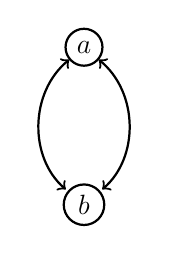
\begin{tikzpicture}[->,shorten >=1pt,auto,node distance=1cm,
        thick,main node/.style={circle,draw,font=\Large\bfseries}]

\tikzstyle{every node}=[draw,shape=circle, scale=0.7];
\node[draw, shape=circle, main node] (1) at (90:1) {$a$} ;
\node[draw, shape=circle, main node] (2) at (270:1) {$b$} ;

\draw[<->] (1) to[bend left=50] (2);
\draw[<->] (1) to[bend right=50] (2);
\end{tikzpicture}
\qquad
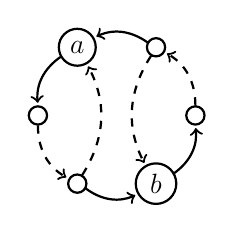
\begin{tikzpicture}[->,shorten >=1pt,auto,node distance=1cm,
        thick,main node/.style={circle,draw,font=\Large\bfseries}]

\tikzstyle{every node}=[draw,shape=circle, scale=0.7];
\node[draw, shape=circle, main node] (1) at (0:1) {} ;
\node[draw, shape=circle, main node] (2) at (60:1) {} ;
\node[draw, shape=circle, main node] (3) at (120:1) {$a$} ;
\node[draw, shape=circle, main node] (4) at (180:1){} ;
\node[draw, shape=circle, main node] (5) at (240:1) {} ;
\node[draw, shape=circle, main node] (6) at (300:1) {$b$} ;

\draw[dashed] (1) to[bend right=30] (2);
\draw[->] (2) to[bend right=30] (3);
\draw[->] (3) to[bend right=30] (4);
\draw[dashed] (4) to[bend right=30] (5);
\draw[->] (5) to[bend right=30] (6);
\draw[->] (6) to[bend right=30] (1);
\draw[dashed] (5) to[bend right=30] (3);
\draw[dashed] (2) to[bend right=30] (6);
\end{tikzpicture} = 
\qquad
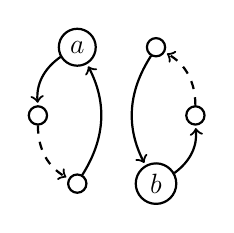
\begin{tikzpicture}[->,shorten >=1pt,auto,node distance=1cm,
        thick,main node/.style={circle,draw,font=\Large\bfseries}]

\tikzstyle{every node}=[draw,shape=circle, scale=0.7];
\node[draw, shape=circle, main node] (1) at (0:1) {} ;
\node[draw, shape=circle, main node] (2) at (60:1) {} ;
\node[draw, shape=circle, main node] (3) at (120:1) {$a$} ;
\node[draw, shape=circle, main node] (4) at (180:1){} ;
\node[draw, shape=circle, main node] (5) at (240:1) {} ;
\node[draw, shape=circle, main node] (6) at (300:1) {$b$} ;

\draw[dashed] (1) to[bend right=30] (2);
\draw[->] (2) to[bend right=30] (6);
\draw[->] (6) to[bend right=30] (1);
\draw[->] (3) to[bend right=30] (4);
\draw[dashed] (4) to[bend right=30] (5);
\draw[->] (5) to[bend right=30] (3);
\end{tikzpicture}
\\

\item
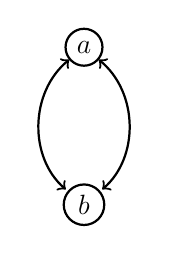
\begin{tikzpicture}[->,shorten >=1pt,auto,node distance=1cm,
        thick,main node/.style={circle,draw,font=\Large\bfseries}]

\tikzstyle{every node}=[draw,shape=circle, scale=0.7];
\node[draw, shape=circle, main node] (1) at (90:1) {$a$} ;
\node[draw, shape=circle, main node] (2) at (270:1) {$b$} ;

\draw[<->] (1) to[bend left=50] (2);
\draw[<->] (1) to[bend right=50] (2);
\end{tikzpicture}
\qquad
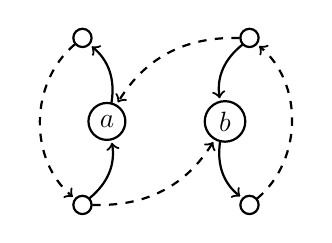
\begin{tikzpicture}[->,shorten >=1pt,auto,node distance=1cm,
        thick,main node/.style={circle,draw,font=\Large\bfseries}]

\tikzstyle{every node}=[draw,shape=circle, scale=0.7];
\node[draw, shape=circle, main node] (1) at (45:1.5) {} ;
\node[draw, shape=circle, main node] (2) at (135:1.5) {} ;
\node[draw, shape=circle, main node] (3) at (225:1.5){} ;
\node[draw, shape=circle, main node] (4) at (315:1.5) {} ;
\node[draw, shape=circle, main node] (5) at (180:.75) {$a$} ;
\node[draw, shape=circle, main node] (6) at (0:.75) {$b$} ;

\draw[->] (1) to[bend right=30] (6);
\draw[dashed] (1) to[bend right=30] (5);
\draw[->] (5) to[bend right=30] (2);
\draw[dashed] (2) to[bend right=50] (3);
\draw[->] (3) to[bend right=30] (5);
\draw[dashed] (3) to[bend right=30] (6);
\draw[->] (6) to[bend right=30] (4);
\draw[dashed] (4) to[bend right=50] (1);
\end{tikzpicture} = 
\qquad
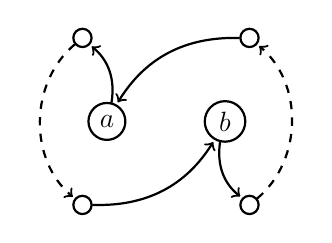
\begin{tikzpicture}[->,shorten >=1pt,auto,node distance=1cm,
        thick,main node/.style={circle,draw,font=\Large\bfseries}]

\tikzstyle{every node}=[draw,shape=circle, scale=0.7];
\node[draw, shape=circle, main node] (1) at (45:1.5) {} ;
\node[draw, shape=circle, main node] (2) at (135:1.5) {} ;
\node[draw, shape=circle, main node] (3) at (225:1.5){} ;
\node[draw, shape=circle, main node] (4) at (315:1.5) {} ;
\node[draw, shape=circle, main node] (5) at (180:.75) {$a$} ;
\node[draw, shape=circle, main node] (6) at (0:.75) {$b$} ;

\draw[->] (1) to[bend right=30] (5);
\draw[->] (5) to[bend right=30] (2);
\draw[dashed] (2) to[bend right=50] (3);
\draw[->] (3) to[bend right=30] (6);
\draw[->] (6) to[bend right=30] (4);
\draw[dashed] (4) to[bend right=50] (1);
\end{tikzpicture}
\\

\item
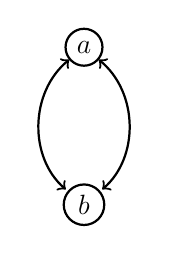
\begin{tikzpicture}[->,shorten >=1pt,auto,node distance=1cm,
        thick,main node/.style={circle,draw,font=\Large\bfseries}]

\tikzstyle{every node}=[draw,shape=circle, scale=0.7];
\node[draw, shape=circle, main node] (1) at (90:1) {$a$} ;
\node[draw, shape=circle, main node] (2) at (270:1) {$b$} ;

\draw[<->] (1) to[bend left=50] (2);
\draw[<->] (1) to[bend right=50] (2);
\end{tikzpicture}
\qquad
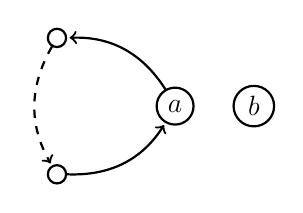
\begin{tikzpicture}[->,shorten >=1pt,auto,node distance=1cm,
        thick,main node/.style={circle,draw,font=\Large\bfseries}]

\tikzstyle{every node}=[draw,shape=circle, scale=0.7];
\node[draw, shape=circle, main node] (1) at (0:1) {$a$} ;
\node[draw, shape=circle, main node] (2) at (120:1) {} ;
\node[draw, shape=circle, main node] (3) at (240:1){} ;
\node[draw, shape=circle, main node] (4) at (0:2) {$b$} ;

\draw[->] (1) to[bend right=30] (2);
\draw[dashed] (2) to[bend right=30] (3);
\draw[->] (3) to[bend right=30] (1);
\end{tikzpicture} = 
\qquad
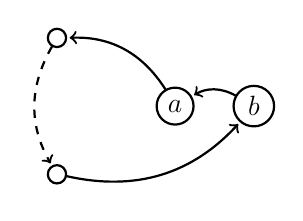
\begin{tikzpicture}[->,shorten >=1pt,auto,node distance=1cm,
        thick,main node/.style={circle,draw,font=\Large\bfseries}]

\tikzstyle{every node}=[draw,shape=circle, scale=0.7];
\node[draw, shape=circle, main node] (1) at (0:1) {$a$} ;
\node[draw, shape=circle, main node] (2) at (120:1) {} ;
\node[draw, shape=circle, main node] (3) at (240:1){} ;
\node[draw, shape=circle, main node] (4) at (0:2) {$b$} ;

\draw[->] (1) to[bend right=30] (2);
\draw[dashed] (2) to[bend right=30] (3);
\draw[->] (3) to[bend right=30] (4);
\draw[->] (4) to[bend right=30] (1);
\end{tikzpicture}
\\

\item
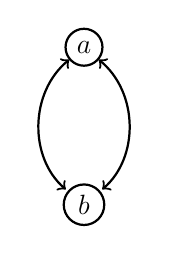
\begin{tikzpicture}[->,shorten >=1pt,auto,node distance=1cm,
        thick,main node/.style={circle,draw,font=\Large\bfseries}]

\tikzstyle{every node}=[draw,shape=circle, scale=0.7];
\node[draw, shape=circle, main node] (1) at (90:1) {$a$} ;
\node[draw, shape=circle, main node] (2) at (270:1) {$b$} ;

\draw[<->] (1) to[bend left=50] (2);
\draw[<->] (1) to[bend right=50] (2);
\end{tikzpicture}
\qquad
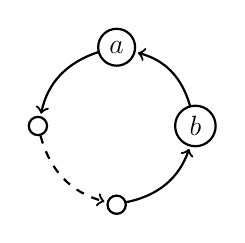
\begin{tikzpicture}[->,shorten >=1pt,auto,node distance=1cm,
        thick,main node/.style={circle,draw,font=\Large\bfseries}]

\tikzstyle{every node}=[draw,shape=circle, scale=0.7];
\node[draw, shape=circle, main node] (1) at (0:1) {$b$} ;
\node[draw, shape=circle, main node] (2) at (90:1) {$a$} ;
\node[draw, shape=circle, main node] (3) at (180:1){} ;
\node[draw, shape=circle, main node] (4) at (270:1) {} ;

\draw[->] (1) to[bend right=30] (2);
\draw[->] (2) to[bend right=30] (3);
\draw[dashed] (3) to[bend right=30] (4);
\draw[->] (4) to[bend right=30] (1);
\end{tikzpicture} = 
\qquad
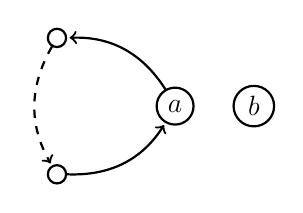
\begin{tikzpicture}[->,shorten >=1pt,auto,node distance=1cm,
        thick,main node/.style={circle,draw,font=\Large\bfseries}]

\tikzstyle{every node}=[draw,shape=circle, scale=0.7];
\node[draw, shape=circle, main node] (1) at (0:1) {$a$} ;
\node[draw, shape=circle, main node] (2) at (120:1) {} ;
\node[draw, shape=circle, main node] (3) at (240:1){} ;
\node[draw, shape=circle, main node] (4) at (0:2) {$b$} ;

\draw[->] (1) to[bend right=30] (2);
\draw[dashed] (2) to[bend right=30] (3);
\draw[->] (3) to[bend right=30] (1);
\end{tikzpicture}
\\

\item
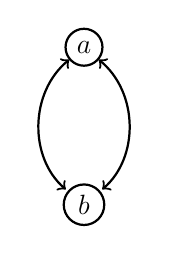
\begin{tikzpicture}[->,shorten >=1pt,auto,node distance=1cm,
        thick,main node/.style={circle,draw,font=\Large\bfseries}]

\tikzstyle{every node}=[draw,shape=circle, scale=0.7];
\node[draw, shape=circle, main node] (1) at (90:1) {$a$} ;
\node[draw, shape=circle, main node] (2) at (270:1) {$b$} ;

\draw[<->] (1) to[bend left=50] (2);
\draw[<->] (1) to[bend right=50] (2);
\end{tikzpicture}
\qquad
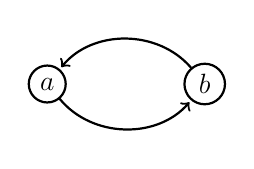
\begin{tikzpicture}[->,shorten >=1pt,auto,node distance=1cm,
        thick,main node/.style={circle,draw,font=\Large\bfseries}]

\tikzstyle{every node}=[draw,shape=circle, scale=0.7];
\node[draw, shape=circle, main node] (1) at (0:1) {$b$} ;
\node[draw, shape=circle, main node] (2) at (180:1) {$a$} ;

\draw[->] (1) to[bend right=50] (2);
\draw[->] (2) to[bend right=50] (1);
\end{tikzpicture} = 
\qquad
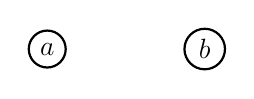
\begin{tikzpicture}[->,shorten >=1pt,auto,node distance=1cm,
        thick,main node/.style={circle,draw,font=\Large\bfseries}]

\tikzstyle{every node}=[draw,shape=circle, scale=0.7];
\node[draw, shape=circle, main node] (1) at (0:1) {$b$} ;
\node[draw, shape=circle, main node] (2) at (180:1) {$a$} ;
\end{tikzpicture}
\\

\item
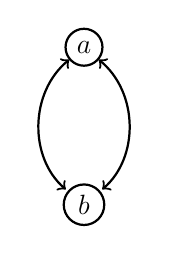
\begin{tikzpicture}[->,shorten >=1pt,auto,node distance=1cm,
        thick,main node/.style={circle,draw,font=\Large\bfseries}]

\tikzstyle{every node}=[draw,shape=circle, scale=0.7];
\node[draw, shape=circle, main node] (1) at (90:1) {$a$} ;
\node[draw, shape=circle, main node] (2) at (270:1) {$b$} ;

\draw[<->] (1) to[bend left=50] (2);
\draw[<->] (1) to[bend right=50] (2);
\end{tikzpicture}
\qquad
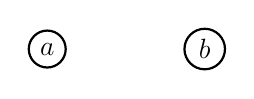
\begin{tikzpicture}[->,shorten >=1pt,auto,node distance=1cm,
        thick,main node/.style={circle,draw,font=\Large\bfseries}]
\tikzstyle{every node}=[draw,shape=circle, scale=0.7];
\node[draw, shape=circle, main node] (1) at (0:1) {$b$} ;
\node[draw, shape=circle, main node] (2) at (180:1) {$a$} ;
\end{tikzpicture} =
\qquad
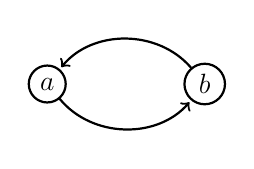
\begin{tikzpicture}[->,shorten >=1pt,auto,node distance=1cm,
        thick,main node/.style={circle,draw,font=\Large\bfseries}]

\tikzstyle{every node}=[draw,shape=circle, scale=0.7];
\node[draw, shape=circle, main node] (1) at (0:1) {$b$} ;
\node[draw, shape=circle, main node] (2) at (180:1) {$a$} ;

\draw[->] (1) to[bend right=50] (2);
\draw[->] (2) to[bend right=50] (1);
\end{tikzpicture}
\end{enumerate}

\noindent\textbf{Exercise  \ref{exercise:Permutations:cycle_length_table}:}
%Using your results from the previous exercise, complete Table~\ref{transposition_table}.
\begin{table}[!htb]
%\caption{Multiplication of permutation by transpositions}\label{transposition_table}
\begin{tabular}{|p{1.6cm}|p{2.7cm}|p{2.7cm}|p{3.5cm}|}
\hline 
\rule{0pt}{2.6ex} Diagram in Fig.~\ref{fig:abC2}&  Change in number of cycles   & Change in sum of cycle lengths & Is column 3 minus column 2 even or odd?  \rule[-1.2ex]{0pt}{0pt} \tabularnewline
\hline
\hline 
\rule{0pt}{2.6ex} (a)  &  +1  & 0  & odd \rule[-1.2ex]{0pt}{0pt} \tabularnewline
\hline 
\rule{0pt}{2.6ex} (b)  &  \underline{-1} & \underline{0} & \underline{odd} \rule[-1.2ex]{0pt}{0pt} \tabularnewline
\hline 
\rule{0pt}{2.6ex} (c)  &  \underline{0} & \underline{1}  & \underline{odd} \rule[-1.2ex]{0pt}{0pt} \tabularnewline
\hline 
\rule{0pt}{2.6ex} (d)  &  \underline{0} & \underline{-1}  & \underline{odd} \rule[-1.2ex]{0pt}{0pt} \tabularnewline
\hline 
\rule{0pt}{2.6ex} (e)  & $-1$ & $-2$ & \underline{odd} \rule[-1.2ex]{0pt}{0pt} \tabularnewline
\hline 
\rule{0pt}{2.6ex} (f)  &  \underline{1} & \underline{2} & \underline{odd}  \rule[-1.2ex]{0pt}{0pt} \tabularnewline
\hline 
\end{tabular}
\end{table}

\noindent\textbf{Exercise  \ref{exercise:Permutations:parity_right}:}\\ %KW need to do
%How does the conclusion of Proposition~\ref{proposition:Permutations:multByTrans} change if the permutation $\sigma$ is multiplied on the \emph{right} by $(ab)$ instead of on the left?  \emph{Explain} your answer.
The conclusion is the same. When multiplying a pair of cycles on the right by a transposition, you either change the number of cycles by 1 or you change the length of one of the cycles by 1. In both cases, the parity changes by 1.

(Note that right multiplication by a transposition gives the very same pictures as in Figures \ref{fig:abC} and \ref{fig:abC2}, only the labelling is changed.)

\noindent\textbf{Exercise  \ref{exercise:Permutations:id_odd}:}\\
%Prove that it is impossible to write the identity permutation as the product of an odd number of transpositions.
Two possible proofs:
\\
Proof (1): When written in disjoint cycle notation, the identity permutation has no cycle lengths and no cycles.  So by the definition of parity, the parity of  $\var{id}$ is $\bmod(0-0,2) = 0$.  By Proposition~\ref{proposition:Permutations:even_and_odd}, it follows that $\var{id}$ is even.\\
\\
Proof (2): Another proof, this time by contradiction.  Suppose that $\var{id}$ can be written as the product of an odd number of transpositions.  Let the first transposition be $(ab)$.  Then $\var{id}$ = $(ab)\tau$, where $\tau$ can be written as an even number of transpositions.  Multiplying both sides on the left by $(ab)$ gives $(ab) = \tau$.  But $(ab)$ is odd and $\tau$ is even, so $(ab)=\tau$ is impossible. This contradiction establishes that $\var{id}$ cannot be written as the product of an odd number of transpositions.\\


\noindent\textbf{Exercise  \ref{exercise:Permutations:even_odd}:}\\
%Suppose $\sigma$ is an $n$-cycle.  How can you tell  whether $\sigma$ is an even or odd permutation?
If $n$ is even, then $\sigma$ is odd; and if $n$ is odd, then $\sigma$ is even.\\

\noindent\textbf{Exercise  \ref{exercise:Permutations:Ex95}:}\\ %KW updated
Recall that an even permutation is any permutation can be written as a product of an even number of transpositions.
\begin{enumerate}[{a.}]
\item
%Prove that the product of two even permutations is even.
Suppose $\sigma$ and $\tau$ are even permutations, then:
	\begin{itemize}
	\item
	$\sigma$ is a product of $2m$ transpositions.

	\item
	$\tau$ is a product of $2n$ transpositions.

	\item
	So $\sigma\tau$ is a product of $(2m+2n)$ transpositions.

	\item
	$\implies$  it's an even permutation.
	\end{itemize}

\item
%Prove that the product of two odd permutations is even.
Suppose $\sigma$ and $\mu$ are odd permutations, then:
	\begin{itemize}
	\item
	$\sigma$ is a product of $2k+1$ transpositions.

	\item
	$\mu$ is a product of $2l+1$ transpositions.

	\item
	So $\sigma\mu$ is a product of $2(l+k+1)$ transpositions.
	
	\item
	$\implies$  it's an even permutation.
	\end{itemize}

\item
%What is the parity of  the product of an even permutation and an odd permutation?  What about the product of an odd permutation and an even permutation? \emph{Prove} your answers.
Let $\tau$ is an even permutation $\implies$  it's a product of $2k$ transpositions.\\
Let $\mu$ is an odd permutation $\implies$  it's a product of $2l+1$ transpositions.\\
$\implies \tau\mu$ is a product of $2(k+l)+1$ transpositions.\\
$\implies$  it's an odd permutation $\implies$  its parity is 1.\\
$\implies \mu\tau$ is a product of $2(l+k)+1$ transpositions.\\
$\implies$  it's an odd permutation $\implies$  its parity is 1.\\
Since the product of an odd permutation and an even permutation will always give you an odd number of transposition, the parity will always be 1.
\end{enumerate}

\noindent\textbf{Exercise  \ref{exercise:Permutations:Sn_even_odd}:}%KW added
%For each of the following sets, describe which permutations are even and which are odd, according to their cycle structure.
%\hyperref[sec:Permutations:Hints]{(*Hint*)}
\begin{enumerate}[(a)]
\item
%$S_6$
\item
%$S_7$
\begin{tabular}{|c|c|c|c|}
	\hline
	Number of Cycles & Legth of cycles & Parity & even or odd \\
 	\hline
  	0(id) & 0 & mod(0,2)=0 & even\\
  	\hline
 	1 & 7 & mod(6,2)=0 & even\\
  	& 6 & mod(5,2)=1 & odd\\
  	& 5 & mod(4,2)=0 & even\\
  	& 4 & mod(3,2)=1 & odd\\
  	& 3 & mod(2,2)=0 & even\\
  	& 2 & mod(1,2)=1 & odd\\
  	\hline
  	2 & 2 and 2 & mod(2,2)=0 & even\\
   & 2 and 3 & mod(3,2)-1 & odd\\
   & 2 and 4 & mod(4,2)=0 & even\\
   & 2 and 5 & mod(5,2)=1 & odd\\
   & 3 and 3 & mod(4,2)=0 & even\\
   & 3 and 4 & mod(5,2)=1 & odd\\
   \hline
  	3 & 2 and 2 and 2 & mod(3,2)=1 & odd\\
   & 2 and 2 and 3 & mod(4,2)=0 & even\\
   \hline
\end{tabular}

\item
%$S_8$
\end{enumerate}

\noindent\textbf{Exercise  \ref{exercise:Permutations:A_nGroupProps}:} %KW added
\begin{enumerate}[(a)]
\item
%Show that ${\var id}  \in A_n$.
In Exercise \ref{exercise:Permutations:id_odd}, we proved that the identity element is an even permutation. Definition \ref{definition:Permutations:defAlternatingGroup} states that $A_{n}$ is the group of all even permutations,\\
$\therefore\ {\var id}\in A_{n}$.

\item
%Show that if $\sigma \in A_n$, then $\sigma^{-1} \in A_n$.
%\hyperref[sec:Permutations:Hints]{(*Hint*)}
Let $\sigma\in A_{n}$ and let $\sigma=\tau_{1}\tau_{2}\cdots\tau_{n-1}\tau_{n}$ for transpositions $\tau_{k}$ for $k=\{1,\dots,n\}$. Now, $\sigma^{-1}=\tau_{1}\tau_{n}\tau_{n-1}\cdots\tau_{2}$.\\
        
$\sigma^{-1}$ has the same transpositions as $\sigma$, therefore it has the same number of cycles and cycle lengths. Which means the parity of $\sigma$ equals the parity of $\sigma^{-1}$. Since $\sigma\in A_{n}$ then $\sigma^{-1}\in A_{n}$.
        
\item
%Show that if $\sigma, \mu \in A_n$, then $\sigma \mu \in A_n$. 
%\hyperref[sec:Permutations:Hints]{(*Hint*)}
Let $\sigma=\tau_{1}\dots\tau_{n}$ and $\mu=\lambda_{1}\dots\lambda_{n}$, then $\sigma\mu=(\tau_{1}\dots\tau_{n})(\lambda_{1}\dots\lambda_{n})$\\

Which is a bunch of products of even permutations and in Exercise \ref{exercise:Permutations:Ex95} we showed that the product of an even permutation with and even permutation is even. Therefore $\sigma\mu\in A_{n}$
\end{enumerate}

\noindent\textbf{Exercise  \ref{exercise:Permutations:B_nGroupProps}:}\\ %KW added
%Prove or disprove: the set of odd permutations $B_n$ is also a group.
In Exercise  \ref{exercise:Permutations:Ex95}(b) we proved that an odd permutation times an odd permutation is even, therefore if you multiply two permutations in $B_{n}$ it would be an even permutation. Therefore $B_{n}$ is not closed under multiplication, which means it is not a group.\\

\noindent\textbf{Exercise  \ref{exercise:Permutations:prove}:}\\

\noindent\textbf{Exercise  \ref{exercise:Permutations:A4}:}\\

\noindent\textbf{Exercise  \ref{exercise:Permutations:A6_A7_A8}:} %KW added
%Give all possible cycle structures for elements in each of the following sets. (You don't need to list all the permutations, just the cycle configurations e.g. ``pair of 2-cycles''.)
\begin{enumerate}[(a)]
\item
%$A_6$

\item
%$A_7$
\begin{center}
\begin{tabular}{|c|c|c|c|}
\hline
Number of Cycles & Legth of cycles & Parity & even or odd \\
\hline
$0(\var{id})$ & $0$ & $\mod(0,2)=0$ & even\\
\hline
$1$ & $7$ & $\mod(6,2)=0$ & even\\
& $5$ & $\mod(4,2)=0$ & even\\
& $3$ & $\mod(2,2)=0$ & even\\
\hline
$2$ & $2$ and $2$ & $\mod(2,2)=0$ & even\\  
& $2$ and $4$ & $\mod(4,2)=0$ & even\\
& $3$ and $3$ & $\mod(4,2)=0$ & even\\
\hline
$3$ & $2$ and $2$ and $3$ & $\mod(4,2)=0$ & even\\
\hline
\end{tabular}
\end{center}

\item
%$A_8$
\end{enumerate}